\documentclass[12pt]{article}
\usepackage{graphicx}
\usepackage{color}

\begin{document}
\begin{titlepage}
\begin{center}
\begin{huge}
\begin{center}
\textcolor{blue}{V3D Digraph Visualizer Documentation}
\end{center}
\end{huge}
\hfill \break
\begin{Large}
\begin{center}
\textcolor{blue}{Team: App-Synth}
\end{center}
\end{Large}
\begin{small}
\begin{flushleft}
Author(s):
\end{flushleft}

\begin{itemize}
	\item Kulani Bamuza \\
	\item Keanan Jones \\
	\item Munyaradzi Mpofu\\
	\item Neo Thokoa\\	
	\item Takalani Sigama\\
	
\end{itemize}
\end{small}

\end{center}
\begin{center}
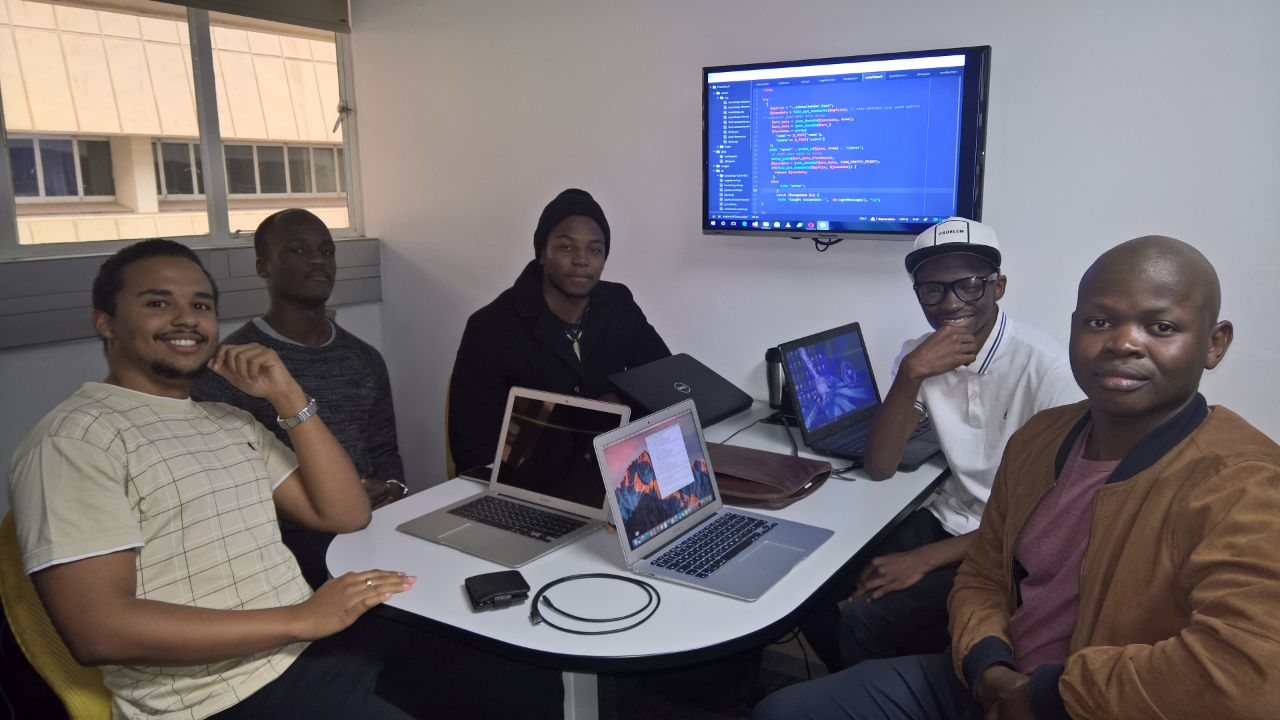
\includegraphics[scale=0.4]{Dps/TeamPic.jpg}
\\
\textcolor{blue}{\textit{University of Pretoria, Department of Computer Science
\\
15 May 2017}}

\end{center}
\end{titlepage}

\newpage
\pagenumbering{arabic}
\thispagestyle{empty}
\tableofcontents
\clearpage

\textcolor{blue}{\section{Introduction}}
\textcolor{blue}{\subsection{Project Background}}
\begin{flushleft}
Graph visualizations allow for humans to perceive the information contained within graph structures in a presentable manner. There exists a number of tools which can be utilised to create 2D visualisations of graph from a single specification. An example of such a tool is GraphViz (insert citation). The aim of this project is to provide the means to generate 3D graphs from a single specification. The graph will then be visualised in a 3D space, which will allow the viewer to immerse themselves within the graph and interact with it.
\end{flushleft}

\textcolor{blue}{\subsection{Project Vision}}
\begin{flushleft}
The increase in performance of graphics engines in this day and age has given rise to many innovative uses of graphics and the development of various graphical applications. The problem which is to be addressed by this project is the design and development of a graphing tool which will visualise a digraph on a plane or a sphere. The viewer of the graph should be able to interact with the digraph and manipulate various aspects of the visualisation.
\end{flushleft}

\textcolor{blue}{\subsection{Project Scope}}
\begin{flushleft}
The system must allow for the visualisation of digraphs which will defined using the set of triples notations as specified by Barla-Szabo (insert citation). The user should be able to change their vantage point while viewing the graph on a hyperplane or hypersphere. The edges of the graph are to be labels using tuples which contain metadata about the edges. This metadata will provide the necessary information required to produce a force directed graph. The users will be immersed in the 3D environment by means of virtual reality 3D glasses. The user should be able to use 3D glasses such as Google Cardboard (insert citation) which they can build themselves in order to make the system more accessible. Besides viewing the graph, the viewer should be able to interact with the graph by manipulating the metadata related to certain vertices and edges. The system should allow for observers to view the 3D environment on an external display.
\end{flushleft}

\textcolor{blue}{\section{Overall Description}}
\textcolor{blue}{\subsection{Product Perspective}}
\begin{flushleft}
The entire system will consist of 2 different applications, namely the desktop application and the mobile application. The mobile application will be deployed on a mobile phone running an android operating system. This application will contain a graphical user interface through which the user can make use of the system. A pair of virtual reality glasses will be required by the user in order to visualise a graph in a 3D space. The mobile application itself will interact with various components of the mobile device, including the camera and the gyroscope. The desktop application will be compatible with Windows, Linux and macOS operating systems. The desktop application will provide observers with a visual representation of the graph being visualized on the mobile device by the user.
\end{flushleft}

\textcolor{blue}{\subsection{Product Function}}
\begin{flushleft}
The system should allow for a predefined graph to be read into the graph visualizer. Once the graph has been loaded, it will be visualised either on a hyperplane or a hypersphere. When the user views the graph, he/she should be able to navigate through the graph by zooming in and out, following the edges between vertices and selecting various topics of interest on the graph. The viewer should be able to set various criteria which will be used for the generation of meta-graphs, such as specifying force direction. The viewer should also be able to edit the graph visualization through the use of hand gestures and the system should provide functionality for the edited graph to be saved as a file in which the graph will be represented as a set of triples. The system should allow for observers to view the graph which is being viewed by the user from the user’s perspective and the visuals which the observers see should be updated accordingly as the user’s viewport changes.
\end{flushleft}

\textcolor{blue}{\subsection{User Characteristics}}
\begin{flushleft}
The typical user groups of the system can be categorised into two different user groups, namely educational professionals such as lecturers and researchers and undergraduate students. Educational professionals may use the graph visualizations to assist with educational activities and the visualizer will also aid researchers in their research activities. For undergraduate students, the graph visualizer will be a useful tool which will assist them in gaining a better understanding of graphs. All of the user groups must have a general understanding of graphs and their various applications. The user must also possess an understanding of certain graph-related concepts such as force direction. The user should possess basic computer literacy skills in order for them to be able to configure and operate the system and they should also be familiar with the environment on which the different components of the system will be deployed eg. Users who intend to make use of the desktop application on a Windows computer should have a general understanding of the Windows OS environment. 
\end{flushleft}

\textcolor{blue}{\subsection{Constraints}}
\begin{flushleft}
The desktop component of the system should be available on multiple platforms, namely Windows, macOS and Linux. The mobile component of the system should be compatible with Android devices. The system itself should be modular to allow for additional functionality to be added as it becomes necessary. 
\end{flushleft}

\textcolor{blue}{\subsection{Assumptions and Dependencies}}
\begin{flushleft}
The devices on which the system is deployed should contain the necessary hardware which is needed for the system to function. Specifically, the mobile device should have a mobile camera, a gyroscope and networking capabilities and the desktop should have networking capabilities and an adequate graphical processing unit. The user will also need to have access to a pair of virtual reality glasses in order to visualize the graphs in a 3D environment.
\end{flushleft}

\textcolor{blue}{\section{User Stories}}
\begin{flushleft}
	The user requirements are derived from a number of user stories. This section serves as a reference to the constructed user stories and under which module they fall under.	
	
	\textcolor{blue}{\subsection{Data Module}}	
	\begin{flushleft}
	\begin{itemize}
	\item As a User, I want to Save Graph for later use
	\item As a User, I want to Update Graph during interaction
	\item As a User, I want to Create Graph from a text file to create a model
	\end{itemize}	
	\end{flushleft}
	
	\textcolor{blue}{\subsection{Interaction Module}}	
	\begin{flushleft}
	\begin{itemize}
	\item As a User, I want to Select Vertex in order to move/edit
	\item As a User, I want to Create Vertex to add to the model
	\item As a User, I want to Update Vertex to a new value
	\item As a User, I want to Remove Vertex from the model
	\item As a User, I want to Create Edge add to the model
	\item As a User, I want to Update Edge to modify forces between vertices to observe structural changes
	\item As a User, I want to Remove Edge from the model
	\end{itemize}	
	\end{flushleft}
	
	\textcolor{blue}{\subsection{Rendering Module}}	
	\begin{flushleft}
	\begin{itemize}
	\item As a User, I want to Render VR Graph for viewing
	\item As a User, I want to Reload Graph to diaplay updated version
	\item As a User, I want to Undo Changes made to graph
	\item As a User, I want to Render Graph on External Display for 3rd party user to view
	\end{itemize}	
	\end{flushleft}
	
	\textcolor{blue}{\subsection{Synchronization Module}}	
	\begin{flushleft}
	\begin{itemize}
	\item As a User, I want to Publish State Changes to sync with external display
	\item As a User, I want to Receive State Changes to sync with VR display
	\end{itemize}	
	\end{flushleft}
	
	
\end{flushleft}

\textcolor{blue}{\section{Functional Product Requirements}}
\begin{flushleft}

	Taking the the user stories in to consideration we will now create a set of product requirements. Each requirement we aim to meet within a sprint (a specified number of days).
	
	\textcolor{blue}{\subsection{Data Module}}	
	\begin{flushleft}
	\begin{itemize}
	\item Read graph data in all specified formats
	\item Format the data in such a way that it is easily interpreted for graph construction
	\item Take graph information and export it to a specified file format
	\end{itemize}	
	\end{flushleft}
	
	\textcolor{blue}{\subsection{Interaction Module}}	
	\begin{flushleft}
	\begin{itemize}
	\item Update graph information through graph interaction
	\item Provide undo functionality on graph
	\end{itemize}	
	\end{flushleft}
	
	\textcolor{blue}{\subsection{Rendering Module}}	
	\begin{flushleft}
	\begin{itemize}
	\item Take formatted graph information and construct a graph
	\item Provide real time rendering from user interactions
	\end{itemize}	
	\end{flushleft}
	
	\textcolor{blue}{\subsection{Synchronization Module}}	
	\begin{flushleft}
	\begin{itemize}
	\item Provide real time rendering on viewer based on VR view
	\item Push relevant changes to external viewers
	\end{itemize}	
	\end{flushleft}

\end{flushleft}

\textcolor{blue}{\section{Non-functional Product Requirements}}
\begin{flushleft}
The system should be able to respond to user actions in a timely manner to allow for smooth user interaction. This requirement is especially vital for user interactions with the graph visualization. There should be real time communication between the mobile application and the desktop application to allow observers to witness the user’s interactions with the graph in real time.

\bigskip

The system must be robust and modular, allowing for simple alterations to the current system and to cater for the future growth of the system by allowing additional features to be implemented and incorporated with ease.

\bigskip

The system should be able to process user input accurately and respond in the appropriate manner at all times.

\bigskip

The system should protect and guide the user to prevent the user from performing any undesirable actions. 

\end{flushleft}

\textcolor{blue}{\section{Use Cases}}
\textcolor{blue}{\subsection{Data Module}}
\begin{flushleft}
UC1.1 Save Graph
\begin{itemize}
\item[i] Description: The system must be able to save any changes which have been made to the graph by the user. Once the graph has been saved, the graph specification should be updated accordingly.
\item[ii] Pre-condition: The graph visualization has been edited.
\item[iii] Post-condition: The changes to the graph specification have been saved.
\end{itemize}
\end{flushleft}

\bigskip

\begin{flushleft}
UC1.2 Update Graph
\begin{itemize}
\item[i] Description: The system should allow for the user to edit an existing graph specification.
\item[ii]	Pre-condition: The required graph specification is selected.
\item[iii] Post-condition: The graph specification has been updated.
\end{itemize}
\end{flushleft}

\bigskip

\begin{flushleft}
UC1.3 Create Graph
\begin{itemize}
\item[i] Description: The system should allow for the user to create a new graph specification to be rendered by the visualizer.
\item[ii] Pre-condition: The option to create a new graph specification is selected.
\item[iii] Post-condition: The graph specification has been created.
\end{itemize}
\end{flushleft}

\includegraphics[scale=0.5]{"Dps/Data Module Actor User Interactions".png}

\bigskip

\textcolor{blue}{\subsection{Interaction Module}}
\begin{flushleft}
UC2.1 Select Vertex
\begin{itemize}
\item[i] Description: The system should allow for the user to select a vertex to interact with through the graph visualization. 
\item[ii] Pre-condition: The user must be viewing the graph in a 3D environment.
\item[iii] Post-condition: The desired vertex has been selected by the user.
\end{itemize}
\end{flushleft}

\bigskip
\begin{flushleft}
UC2.2 Create Vertex
\begin{itemize}
\item[i] Description: The system should allow for the user to create a new vertex and add it to the graph visualization.
\item[ii] Pre-condition: The user must be viewing the graph in a 3D environment.
\item[iii] Post-condition: A vertex has been added to the graph.
\end{itemize}
\end{flushleft}

\bigskip

\begin{flushleft}
UC2.3 Update Vertex
\begin{itemize}
\item[i] Description: The system should allow for the user to update any metadata related to a particular vertex.
\item[ii] Pre-condition: The user must be viewing the graph in a 3D environment.
\item[iii] Post-condition: The desired vertex has been updated.
\end{itemize}
\end{flushleft}

\bigskip

\begin{flushleft}
UC2.4 Remove Vertex
\begin{itemize}
\item[i] Description: The system should allow for the user to remove a vertex from the graph visualization.
\item[ii] Pre-condition: The user must be viewing the graph in a 3D environment.
\item[iii] Post-condition: A vertex has been removed from the graph.
\end{itemize}
\end{flushleft}
\bigskip

\begin{flushleft}
UC2.5 Create Edge
\begin{itemize}
\item[i] Description: The system should allow for the user to create a new edge and add it to the graph visualization.
\item[ii] Pre-condition: The user must be viewing the graph in a 3D environment.
\item[iii] Post-condition: A vertex has been added to the graph.
\end{itemize}
\end{flushleft}

\bigskip

\begin{flushleft}
UC2.6 Update Edge
\begin{itemize}
\item[i] Description: The system should allow for the user to update any metadata related to a particular edge.
\item[ii] Pre-condition: The user must be viewing the graph in a 3D environment.
\item[iii] Post-condition: The desired vertex has been updated.
\end{itemize}
\end{flushleft}

\bigskip

\begin{flushleft}
UC2.7 Remove Edge
\begin{itemize}
\item[i] Description: The system should allow for the user to remove an edge from the graph visualization.
\item[ii] Pre-condition: The user must be viewing the graph in a 3D environment.
\item[iii] Post-condition: A vertex has been removed from the graph.
\end{itemize}
\end{flushleft}

\includegraphics[scale=0.5]{"Dps/Interaction Module Actor User Interactions".png}

\textcolor{blue}{\subsection{Rendering Module}}

\begin{flushleft}
UC3.1 Render VR Graph
\begin{itemize}
\item[i] Description: The system should provide the functionality to render a graph visualization. The visualization will be constructed based on a graph specification provided by the user.
\item[ii] Pre-condition: A graph specification must be provided by the user.
\item[iii] Post-condition: A graph visualisation has been rendered by the system.
\end{itemize}
\end{flushleft}

\bigskip

\begin{flushleft}
UC3.2 Reload Graph
\begin{itemize}
\item[i] Description: The system should allow for a graph visualisation to be re-rendered. The graph visualisation will be reconstructed based on the latest available graph specification.
\item[ii] Pre-condition: The graph specification must be valid.
\item[iii] Post-condition: The graph has been re-rendered.
\end{itemize}
\end{flushleft}

\bigskip

\begin{flushleft}
UC3.3 Undo Changes
\begin{itemize}
\item[i] Description: The system should allow for the user to undo any changes which have been made to the graph visualization.
\item[ii] Pre-condition: The user must be viewing the graph in a 3D environment.
\item[iii] Post-condition: The graph has been reverted to a valid previous state.
\end{itemize}
\end{flushleft}

\bigskip

\begin{flushleft}
UC3.4 Render Graph on External Display
\begin{itemize}
\item[i]Description: The system should provide the functionality to render a graph on an external display. The graph rendered on the external display will be constructed based on the graph which is rendered by the graph visualizer on the mobile device.
\item[ii] Pre-condition: A graph visualization should be rendered on the mobile device.
\item[iii] Post-condition: A graph has been rendered on the external display.
\end{itemize}
\end{flushleft}

\includegraphics[scale=0.5]{"Dps/Rendering Actor System Interactions".png}

\textcolor{blue}{\subsection{Synchronization Module}}
\begin{flushleft}
UC4.1 Publish State Changes
\begin{itemize}
\item[i] Description: The system should allow for the mobile application to publish any graph state changes to the desktop application. 
\item[ii] Pre-condition: The mobile application and the desktop applications should have a means of communication.
\item[iii] Post-condition: The state changes have been pushed to the desktop application.
\end{itemize}
\end{flushleft}

\begin{flushleft}
UC4.2 Receive State Changes
\begin{itemize}
\item[i]Description: The system should allow for the desktop application to receive the graph state changes which have been published by the mobile application.
\item[ii] Pre-condition: The mobile application and the desktop applications should have a means of communication.
\item[iii] Post-condition: The state changes have been received by the desktop application and the graph on the external display has been updated accordingly.
\end{itemize}
\end{flushleft}

\includegraphics[scale=0.5]{"Dps/Sync Actor System Interactions".png}

\textcolor{blue}{\section{Business Value vs Technical Difficulty \& Product Backlog}}
\begin{flushleft}
 	
 	The product requirements are plotted on the following graph to illustrate how important they are for business success and how difficult each is to implement.
	
	\includegraphics[scale=0.5]{"Deployment Diagrams/businessValueVsTechnicalDifficulty".png}
	
	According to the diagram and fulfilling as many prerequisites as possibly while maintaining concurrency we have the following implementation order on the product backlog.
	
	\includegraphics[scale=0.6]{"Deployment Diagrams/productBacklog".png}

\end{flushleft}

\begin{flushleft}

	We use the order of cards in the backlog as a guide to help us order our execution order. Taking into account other factors such as dependencies. The execution order are reflected in the burndown charts as well as how we conduct our sprints.
	
\end{flushleft}

\end{document}